%        File: planoic.tex
%     Created: Fri Apr 18 01:00 PM 2014 B
% Last Change: Fri Apr 18 01:00 PM 2014 B
%
\documentclass[12pt, a4paper, oneside]{article}

\usepackage{amsfonts}
\usepackage[]{amsmath}
\usepackage{amssymb}
\usepackage[brazil]{babel}
\usepackage[left=20mm,right=20mm,top=25mm,bottom=25mm]{geometry}
\usepackage[]{graphicx}
\usepackage[utf8]{inputenc}
\usepackage{multirow}
\usepackage{paralist}
\usepackage{setspace}
\usepackage[compact]{titlesec}
\usepackage[]{url}
\usepackage{xspace}
\usepackage{mathpazo}
\usepackage{txfonts}

%\usepackage[]{biblatex}

\titleformat{\section}
  {\Large\bfseries}{\thesection.}{.5em}{}[\hrule\bigskip]
\titleformat{\subsection}
  {\bfseries}{\thesection.}{.5em}{}
%\renewcommand{\baselinestretch}{1.5} 
%\renewcommand{\rmdefault}{phv} % Arial
%\renewcommand{\sfdefault}{phv} % Arial
\setlength{\parskip}{6pt}

\newcommand{\A}{\ensuremath{\mathtt{A}}\xspace}
\newcommand{\C}{\ensuremath{\mathtt{C}}\xspace}
\newcommand{\G}{\ensuremath{\mathtt{G}}\xspace}
\newcommand{\T}{\ensuremath{\mathtt{T}}\xspace}

\newcommand{\str}[1]{\ensuremath{\mathtt{#1}}\xspace}
\newcommand{\strset}[1]{\ensuremath{\mathcal{#1}}\xspace}
\newcommand{\ssS}{\strset{S}}
\newcommand{\seq}[1]{\ensuremath{\mathtt{#1}}\xspace}

\newcommand{\rank}{\ensuremath{\mathrm{rank}}\xspace}
\newcommand{\select}{\ensuremath{\mathrm{select}}\xspace}
\newcommand{\BWT}{\ensuremath{\mathrm{BWT}}\xspace}

\newcommand{\X}{\ensuremath{\medbullet}\xspace}
\newcommand{\x}{\ensuremath{\medcirc}\xspace}


%\bibliography{projeto}


\begin{document}
%\onehalfspacing

%\maketitle

\thispagestyle{empty}
\begin{center}
\Large
Universidade Federal de Pernambuco\\
Centro de Informática\\
Graduação em Engenharia da Computação

\vfill

{\huge \bfseries Estruturas de índices sucintas para grafos de subsequencias}
\\
\medskip
{\bfseries\itshape Proposta de Trabalho de Graduação}

\vfill

\bigskip

	\begin{tabular}{r p{95mm}}
	\textbf{Aluno: } & Vitor Travassos Castelo Branco\newline(\texttt{vtcb@cin.ufpe.br}) \\ 
\textbf{Orientador: } & Paulo Gustavo Soares da Fonseca \newline(\texttt{paguso@cin.ufpe.br})
\\
	\textbf{Área: } & Teoria da Computação / Algoritmos
\end{tabular}

	\vspace{3cm}
Recife, 04 de Abril de 2018
\end{center}

\clearpage 
\thispagestyle{empty}
\section{Resumo}
Boa parte das ferramentas para o sequenciamento do DNA baseado nas plataformas de alto desempenho ditas de nova geração, especificamente as destinadas à montagem dos fragmentos sequenciados, utilizam estruturas de dados para grafos de subsequencias. Devido ao enorme volume de dados, um dos principais gargalos dessas representações é espaço em memória exigido. Várias representações compactas vêm sendo propostas nos últimos anos. Entretanto, existe uma relação inversa entre o espaço de memória e a eficiência/flexibilidade das operações suportadas. Mais recentemente, têm-se explorado a conexão entre os grafos de subsequencias e os índices de texto. Neste projeto, pretendemos produzir uma implementação dos Grafos de de Bruijn baseada numa representação sucinta da árvore de sufixos. Essa implementação será analisada e comparada a alternativas disponíveis na literatura para aferir a sua viabilidade em termos de espaço e tempo.

\clearpage
\setcounter{page}{1}
\section{Introdução}

%O DNA, molécula orgânica responsável pela codificação e transmissão das características ge\-né\-ti\-cas, é constituído por duas cadeias complementares formadas a partir de quatro \emph{bases nitrogenadas}, representadas por \A, \C, \G e \T. Cada \A de uma cadeia (fita) é emparelhado a um \T da outra, assim como cada \G é complementado por um \C, e vice versa. Essa estrutura molecular torna-o passível de representação por apenas uma sequência de letras no alfabeto dessas quatro letras. Desvendar o genoma de um organismo limita-se com identificar a sequência de caracteres correspondente ao seu DNA. 

Atualmente, o processo de sequenciamento de DNA é efetuado principalmente utilizando-se as plataformas de sequenciamento de alto desempenho ditas de ``nova geração'' (\textit{Next-Generation Sequencing---NGS}) \cite{Pop2008}. Essas tecnologias produzem um enorme volume de fragmentos curtos (comprimento abaixo das centenas) que precisam ser \emph{montados}, i.e., alinhados e combinados, para reconstruir sequências originais de bilhões de letras.

As ferramentas para montagem de fragmentos NGS são majoritariamente baseadas nos chamados \emph{Grafos de de Bruijn} (GDB) \cite{Compeau2011}. No GDB de ordem $k$ construído a partir do conjunto de fragmentos $\ssS$, $G(\ssS)$, os nós correspondem às subsequencias de comprimento $k$ ($k$-mers) das cadeias em \ssS, e dois $k$-mers (nós) são unidos por uma aresta desde que haja uma sobreposição de tamanho $k-1$, de forma que as arestas correspondem aos $k+1$-mers de \ssS.  Efetuar a montagem de fragmentos usando GDB envolve problemas como o de encontrar \emph{Caminhos Eulerianos}, que admite solução em tempo polinomial. Entretanto, um dos principais limitadores quanto ao emprego dessas técnicas é o espaço de memória exigido pelos GDB que, se representado explicitamente, pode requerer centenas de GigaBytes \cite{Conway2011}. Diante disto, diversos esforços vêm sendo empreendidos para desenvolver estruturas de dados eficientes do ponto de vista de espaço, permitindo todavia operações sobre o GDB em tempo comparável a uma representação tradicional.

%\begin{figure}
%	\begin{center}
%	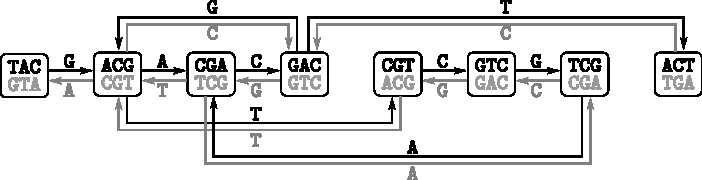
\includegraphics{dbg}
%	\end{center}
%	\caption{GDB de ordem $k=3$ da cadeia $S=\str{TACGACGTCGACT}$. Os nós são rotulados pelos 3-mers (em preto) e temos uma aresta dirigida $x_0x_1x_2\stackrel{y_2}\longrightarrow y_0y_1y_2$ sempre que $x_1x_2=y_0y_1$. Ocorre que, no sequenciamento de DNA, normalmente não sabemos se foi lida a sequência de uma fita ou da sua complementar, no sentido oposto. Portanto, o 4-mer $x_0x_1x_2x_3$ tanto pode representar a aresta $x_0x_1x_2\stackrel{x_3}\longrightarrow x_1x_2x_3$ como a aresta $x'_3x'_2x'_1\stackrel{x'_0}\longrightarrow x'_2x'_1x'_0$ ($x'j$ denota a base complementar de $x_j$). Por essa razão é comum identificar o nó ($k$-mer) com seu complemento reverso (em cinza) e considerar o grafo como bidirecional.}  \label{fig:dbg}
%\end{figure}

A representação e manipulação de GDB envolve técnicas algorítmicas específicas que visam a minimisar o uso de memória principal. Essas técnicas incluem o desenho de algoritmos otimizados para memória externa/cache, o desenvolvimento de \emph{estruturas de dados sucintas} \cite{Jacobson1989}, e o uso de compressão de dados.
Os métodos  descritos na literatura procuram representar ou o conjunto de vértices ($k$-mers) ou arestas ($K+1$-mers) com estruturas de dados específicas de forma a permitir que as operações de navegação como `quais são os sucessores/predecessores de um nó $v$?' sejam respondidas indiretamente através de operações primitivas de baixo nível. 

Num dos primeiros esforços, Conway e Bromage \cite{Conway2011} propuseram-se a representar $G(\ssS)$ a partir do seu conjunto de arestas $E$ como um conjunto de $k+1$-mers ordenados lexicograficamente. Cada uma das possíveis arestas pode ser identificada com uma posição de um bit array comprimido  \cite{Okanohara2007}. 
Operações de navegação como são realizadas através de consultas ao bit array.
Os autores obtiveram assim cerca de 28 bits por aresta para o GDB do genoma de um humano.


Pell et al \cite{Pell2012} propuseram uma representação mais econômica que consiste em armazenar o conjunto dos vértices $V$ ($k$-mers) de  $G(\ssS)$ num \emph{Filtro de Bloom (FB)} \cite{Bloom1970}.
Apesar de consultas ao FB poderem retornar falsos-positivos, Pell et al sustentam que a representação mantém propriedades 
adequadas para tarefas como a decomposição do GDB em componentes para a posterior montagem de trechos contíguos (\emph{contigs}) da sequência original.   
Chikhi e Rizk \cite{Chikhi2013} estenderam a representação de Pell ara representar explicitamente um conjunto de \emph{falsos-positivos críticos} (FPc). Com isso, obteve-se uma representação exata que permitiu que o GDB do genoma humano (HapMap: NA18507) fosse armazenado em cerca de 6~GigaBytes. Posteriormente, essa estrutura foi refinada por Salikhov et al \cite{Salikhov2014} com a utilização em cascata de FB para representar o conjunto de FPc (ao invés de hash tables), obtendo uma representação cerca de 30--40\% mais eficiente em termos de memória, e 18--30\% em termos de tempo de percurso do GDB.

A representação apresentada por Bowe et al \cite{Bowe2012} foi inspirada pela \emph{Transformada de Burrows-Wheeler} (BWT) \cite{Burrows1994}. 
A BWT é uma permutação de um texto que permite a compressão e a busca eficiente por padrões sobre ele. Bowe et al propuseram representar o GDB de uma cadeia $S$ de comprimento $n$ como uma permutação $W$ similar à sua BWT. Essa cadeia, juntamente com um bit array de tamanho $n$ e mais as contagens de cada caractere em $S$, permitem a navegação sobre o GDB. No total, essa representação do GDB requer cerca de 2.5~GigaBytes para o mesmo data set do genoma humano (HapMap: NA18507) mencionado acima.
Boucher et al \cite{Boucher2015} estenderam a representação de \cite{Bowe2012} para permitir operações de navegação com o $k$ variável e escolhido \emph{on-the-fly}. Belazzougui et al \cite{Belazzougui2016} refinaram ainda mais a re\-pre\-sen\-ta\-ção de \cite{Boucher2015}, introduzindo, uma estrutura bidirecional \cite{Schnattinger2012}. Essa modificação tem um custo acrescido de $O(n\lg k)$ bits de espaço ($n=$número de vértices) sobre a representação base de \cite{Bowe2012}, permitindo todavia navegar sobre o GDB nos dois sentidos e com $k$ variável em tempo $O(\lg k)$ por aresta. 

Outras propostas de representação são baseadas \emph{FM-index} \cite{Ferragina2000}, que é uma extensão sucinta da BWT. R{\o}dland \cite{Rodland2013} propôs uma variação do FM-index, chamado $k$FM-index, para representar diretamente o conjunto de $k+1$-mers (arestas) de um conjunto de sequências em ordem lexicográfica. Essa representação requer cerca de 5 bits por nó, o que é suficiente para permitir a navegação no GDB no sentido reverso das arestas.
Chikhi et al \cite{Chikhi2015} também propuseram uma representação chamada DBGFM que consiste em representar através de um FM-index a cadeia correspondente à concatenação dos rótulos das arestas de todos os \emph{caminhos simples maximais} (i.e. contendo apenas nós sem bifurcação) de $G(\ssS)$. A implementação de \cite{Chikhi2015} usa ainda a codificação de Huffman para comprimir a BWT, demandando apenas $\approx 1.5$~GigaBytes para o data set NA18507 do genoma humano referido anteriormente. 

Embora os métodos anteriores já evidenciem a relação entre os GDB e as estruturas de índice, Cazaux et al \cite{Cazaux2016} propuseram-se a investigar mais aprofundadamente essa conexão, em particular com as árvores de sufixos, que é um índice de referência muito estudado \cite{Apostolico1985}. Nesse estudo teórico, os autores apresentaram algoritmos lineares para a construção de GDB a partir de árvores de sufixos, árvores de sufixos truncadas \cite{Na2003}, e arrays de sufixos \cite{Manber1993}. Essa estratégia pode tirar proveito da construção prévia de um desses índices para uma outra tarefa, como a correção de erros de sequenciamento, por exemplo.


\clearpage
\section{Objetivos}

Conforme visto acima, o tema deste projeto é um tópico ativo de pesquisa com muitas contribuições recentes. Apesar da literatura relativamente extensa, os desenvolvimentos ainda não estão consolidados. Em particular, observa-se uma grande disparidade metodológica nas abordagens, com diversas estruturas sendo adotadas. Essas estruturas refletem as necessidades e objetivos particulares dos estudos e das ferramentas para as quais foram desenvolvidas, e implementam portanto um conjunto não-uniforme de funcionalidades. Além disso, as estruturas apresentam níveis muito distintos de maturidade, algumas delas já bem integradas em ferramentas mais estáveis e.g.  \cite{Chikhi2013, Salikhov2014}, outras ainda em fase de protótipo, e.g. \cite{Bowe2012, Rodland2013}, e outras para as quais não conhecemos implementações, e.g.\cite{Cazaux2016}.

O principal objetivo deste projeto é explorar a conexão teórica entre os GDB e as estruturas de índices, e sua realização prática. Em particular, o recente trabalho de Cazaux et al \cite{Cazaux2016} aponta para as conexões entre as árvores de sufixos e os GDB. Neste trabalho iremos desenvolver uma implementação sucinta baseada em Árvores de Sufixos Comprimidas \cite{Sadakane2007}. Esta implementação será avaliada do ponto de vista teórico e prático quanto ao (i)~tempo e memória de construção da estrutura, (ii)~espaço de memória final da estrutura, (iii)~tempo das operações de navegação através da simulação de percursos no grafo. Os resultados serão comparados a outras implementações mencionadas acima.

%Todavia, a estrutura proposta é assimétrica, no sentido discutido em \cite{Belazzougui2016}, pelo que um um outro objetivo específico que podemos apontar seria estender essa conexão para estruturas bidirecionais como as árvores e/ou arrays de afixos \cite{Maass2003, Strothmann2007}. Além disso, como mencionado acima, \cite{Cazaux2016} contém um estudo teórico sobre os algoritmos para a conversão de árvores e arrays de sufixos em GDB. Também temos como objetivo investigar as implementações eficientes para os GDB assim obtidos, tendo por base representações sucintas para as árvores de sufixos \cite{Sadakane2007}.

O software desenvolvido no projeto será acrescentado a uma biblioteca básica em escrita em C, atualmente em desenvolvimento, para que possa ser útil à comunidade de processamento de texto e Biologia Computacional.


\clearpage
\section{Metodologia}

O projeto será organizado nas atividades descritas abaixo e desenvolvidas conforme o cronograma a seguir.

\subsection{T0. Preparação da proposta}

Nesta fase inicial, aluno e orientador farão uma série de reuniões para definição do problema e escopo do projeto. O orientador apresentará a bibliografia básica sobre o tema e os possíveis pontos a serem abordados, e ambos decidirão sobre aqueles a serem desenvolvidos com base no  interesse mútuo.

\subsection{T1. Revisão e acompanhamento bibliográfico}

Essa tarefa será executada de maneira mais acentuada no início do projeto. A atividade consiste num estudo dirigido centrado no  material bibliográfico mais diretamente relacionado às estruturas de dados e algoritmos a serem implementados no projeto. Ao final dessa fase inicial, espera-se que o aluno possa manter-se atualizado e aprofundar-se em pontos específicos de maneira mais autônoma.


\subsection{T2. Implementação das estruturas}

Esta tarefa corresponde à principal componente de desenvolvimento do projeto. O aluno deverá, em interação com o orientador, estudar detalhadamente algoritmos e estruturas de dados relativos aos índices e grafos de subsequências, e desenvolver uma implementação de referência em nível de produção para os mesmos, com base em uma biblioteca em C atualmente em desenvolvimento.


\subsection{T3. Realização dos Testes}

Nesta tarefa, o aluno deverá fazer uma análise experimental comparativa do desempenho dos métodos propostos e implementados relativamente a outras alternativas públicas identificadas num levantamento inicial na tarefa T1. Pode ser necessário obter dados reais e produzir dados sintéticos que simulem uma situação limite de estresse para os métodos.


\subsection{T4. Redação e revisão da monografia}

A monografia produzida deverá conter:
(1)~uma breve revisão bibliográfica do estado da arte, fruto da tarefa T1, (2)~descrição detalhada dos seus desenvolvimentos, incluindo a análise teórica dos algoritmos e estruturas propostas em termos de tempo e espaço, (3)~uma análise crítica com base em resultados experimentais da tarefa T3, e (4)~uma discussão com conclusões gerais sobre o projeto.


\subsection{T5. Preparação da Apresentação}

Finalmente, o aluno preparará a apresentação da defesa do TG com o resumo dos desenvolvimentos e resultados obtidos.

\medskip

O aluno já possui alguma familiaridade com a área, tendo inclusive cursado uma disciplina eletiva oferecida pelo orientador, pelo que poderá por-se rapidamente em desenvolvimento. O acompanhamento será feito pessoalmente através de reuniões semanais. Todo material desenvolvido é compartilhado entre orientador e aluno através de um repositório privado na plataforma GitHub. 


\clearpage
\section{Cronograma de atividades}


\begin{center}
	\begin{tabular}{| l || c | c | c | c | c | c | c | c | c | c | c | c | c | c | c |  c | c | c | c | }
		\hline
		& \multicolumn{2}{| c |}{Mar} & \multicolumn{4}{| c |}{Abr} & \multicolumn{4}{| c |}{Mai} & \multicolumn{4}{| c |}{Jun} & \multicolumn{2}{| c |}{Jul} \\\hline\hline
		Preparação da proposta & \X & \X & & & & & & & & & & & & & & \\\hline 
		Revisão bibliográfica$^\dagger$ & \X & \X & \x & \x & \x & \x & \x & \x & & & & & & & & \\\hline 
		Implementação das estruturas & & & \X & \X & \X & \X & \X & \X & \X & \X & \X & & & & & \\\hline 
		Realização dos testes$^\ddagger$ & & & & \x & \x & \x & \x & \x & \x  & \X & \X & \X & & & & \\\hline 
		Redação e revisão da monografia & & & & & & & & & & & \X & \X & \X & \X & & \\\hline 
		Preparação da apresentação & & & & & & & & & & & & & & & \X & \X \\\hline 
\hline
	\end{tabular}
\begin{minipage}{0.6\linewidth}
\noindent($\dagger$) \X = levantamento inicial, \x= aprofundamento\newline
\noindent($\ddagger$) \X= experimentos formais , \x = testes \textit{ad hoc} unitários\newline
\end{minipage}

\end{center}


\clearpage
%\nocite{*}
\bibliographystyle{unsrt-etal}
\bibliography{proposta}
%\printbibliography

\clearpage
\section{Possíveis Avaliadores}

\begin{enumerate}
\item Profa. Katia  Guimarães
\item Prof. Pedro Manhães
\end{enumerate}


\clearpage
\section{Assinaturas}

\vfill
\begin{center}
	Recife, 04 de Abril de 2018

	\vspace{3cm}
	\rule{10cm}{.5pt}\\
	\textbf{Aluno:} Vitor Travassos Castelo Branco\\

	\vspace{3cm}
	\rule{10cm}{.5pt}\\
	\textbf{Orientador:} Paulo Gustavo Soares da Fonseca\\
\end{center}
\vfill

\end{document}

